\documentclass{beamer}
\usepackage[utf8]{inputenc}
\usepackage[russian]{babel}
\usepackage{graphicx} % Для работы с изображениями
\usepackage{amsmath}  % Для формул
\usepackage{hyperref} % Для ссылок
\usepackage{xcolor}   % Для настройки цветов

\definecolor{custom_green}{RGB}{44, 134, 92}
% Настройка стиля презентации
\usetheme{Goettingen} % Можно заменить на другой стиль

\title[Информатика]{Информатика 2023-2024}
\subtitle{Лекция 2 Целые числа со знаком в трёхразрядном компьютере}
\author{Балакшин Павел Валерьевич}
\date{\today}

\begin{document}

% Первый слайд: Титульный
\begin{frame}
    \titlepage
\end{frame}

% Второй слайд
\begin{frame}{Решение проблемы с округлением в СС с чётным основанием}
    Суть решения — использовать неклассические правила округления:
    \begin{itemize}
        \item \textcolor{custom_green}{Случайное округление}: используется датчик случайных чисел при принятии решения о том, в бóльшую или меньшую сторону следует округлять.
        \item \textcolor{custom_green}{Банковское округление} (к ближайшему чётному): \(3,5\approx4\), но \(2,5\approx2\).
        \item \textcolor{custom_green}{К ближайшему нечётному}: \(3,5\approx3\), но \(2,5\approx3\). Аналогично \(4,3_{(6)}\approx5_{(6)}\).
        \item \textcolor{custom_green}{Чередующееся}: направление округления меняется на противоположное при каждой операции округления (необходимо <<помнить>> о предыдущем округлении).
    \end{itemize}
    \textbf{Примечание.} Каждое из правил можно применять как полностью универсально, так и комбинировано с классическим правилом округления, дополняя его лишь при округлении пограничных значений.
\end{frame}

% Третий слайд
\begin{frame}{Пример округления}
    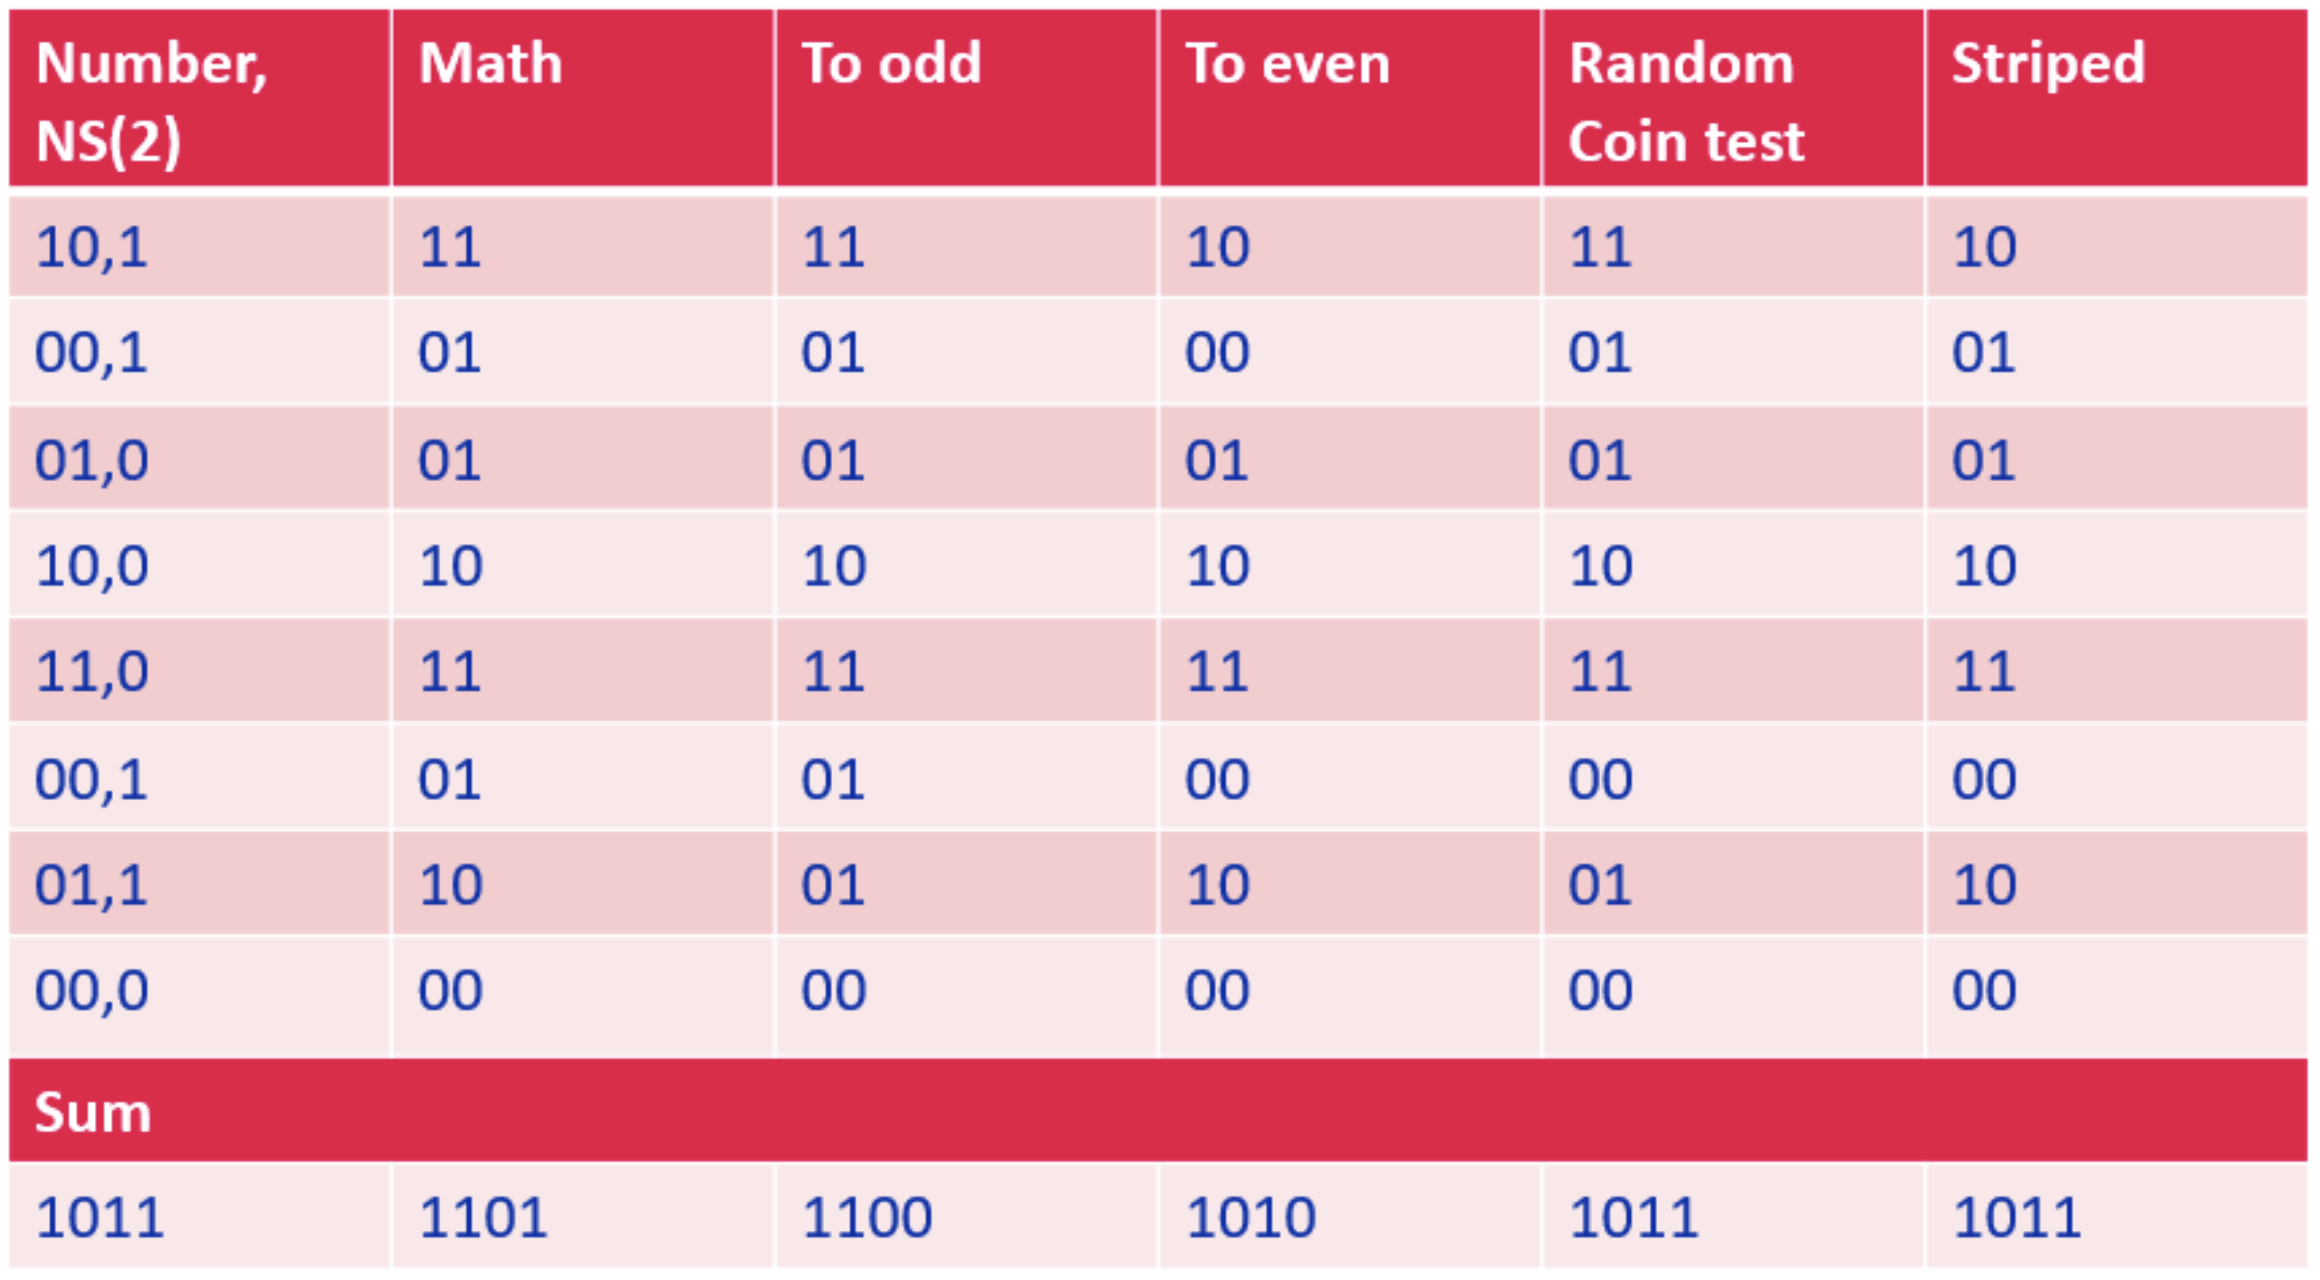
\includegraphics[width=\textwidth]{1.png}
\end{frame}

% Четвёртый слайд
\begin{frame}{Пример округления (2)}
    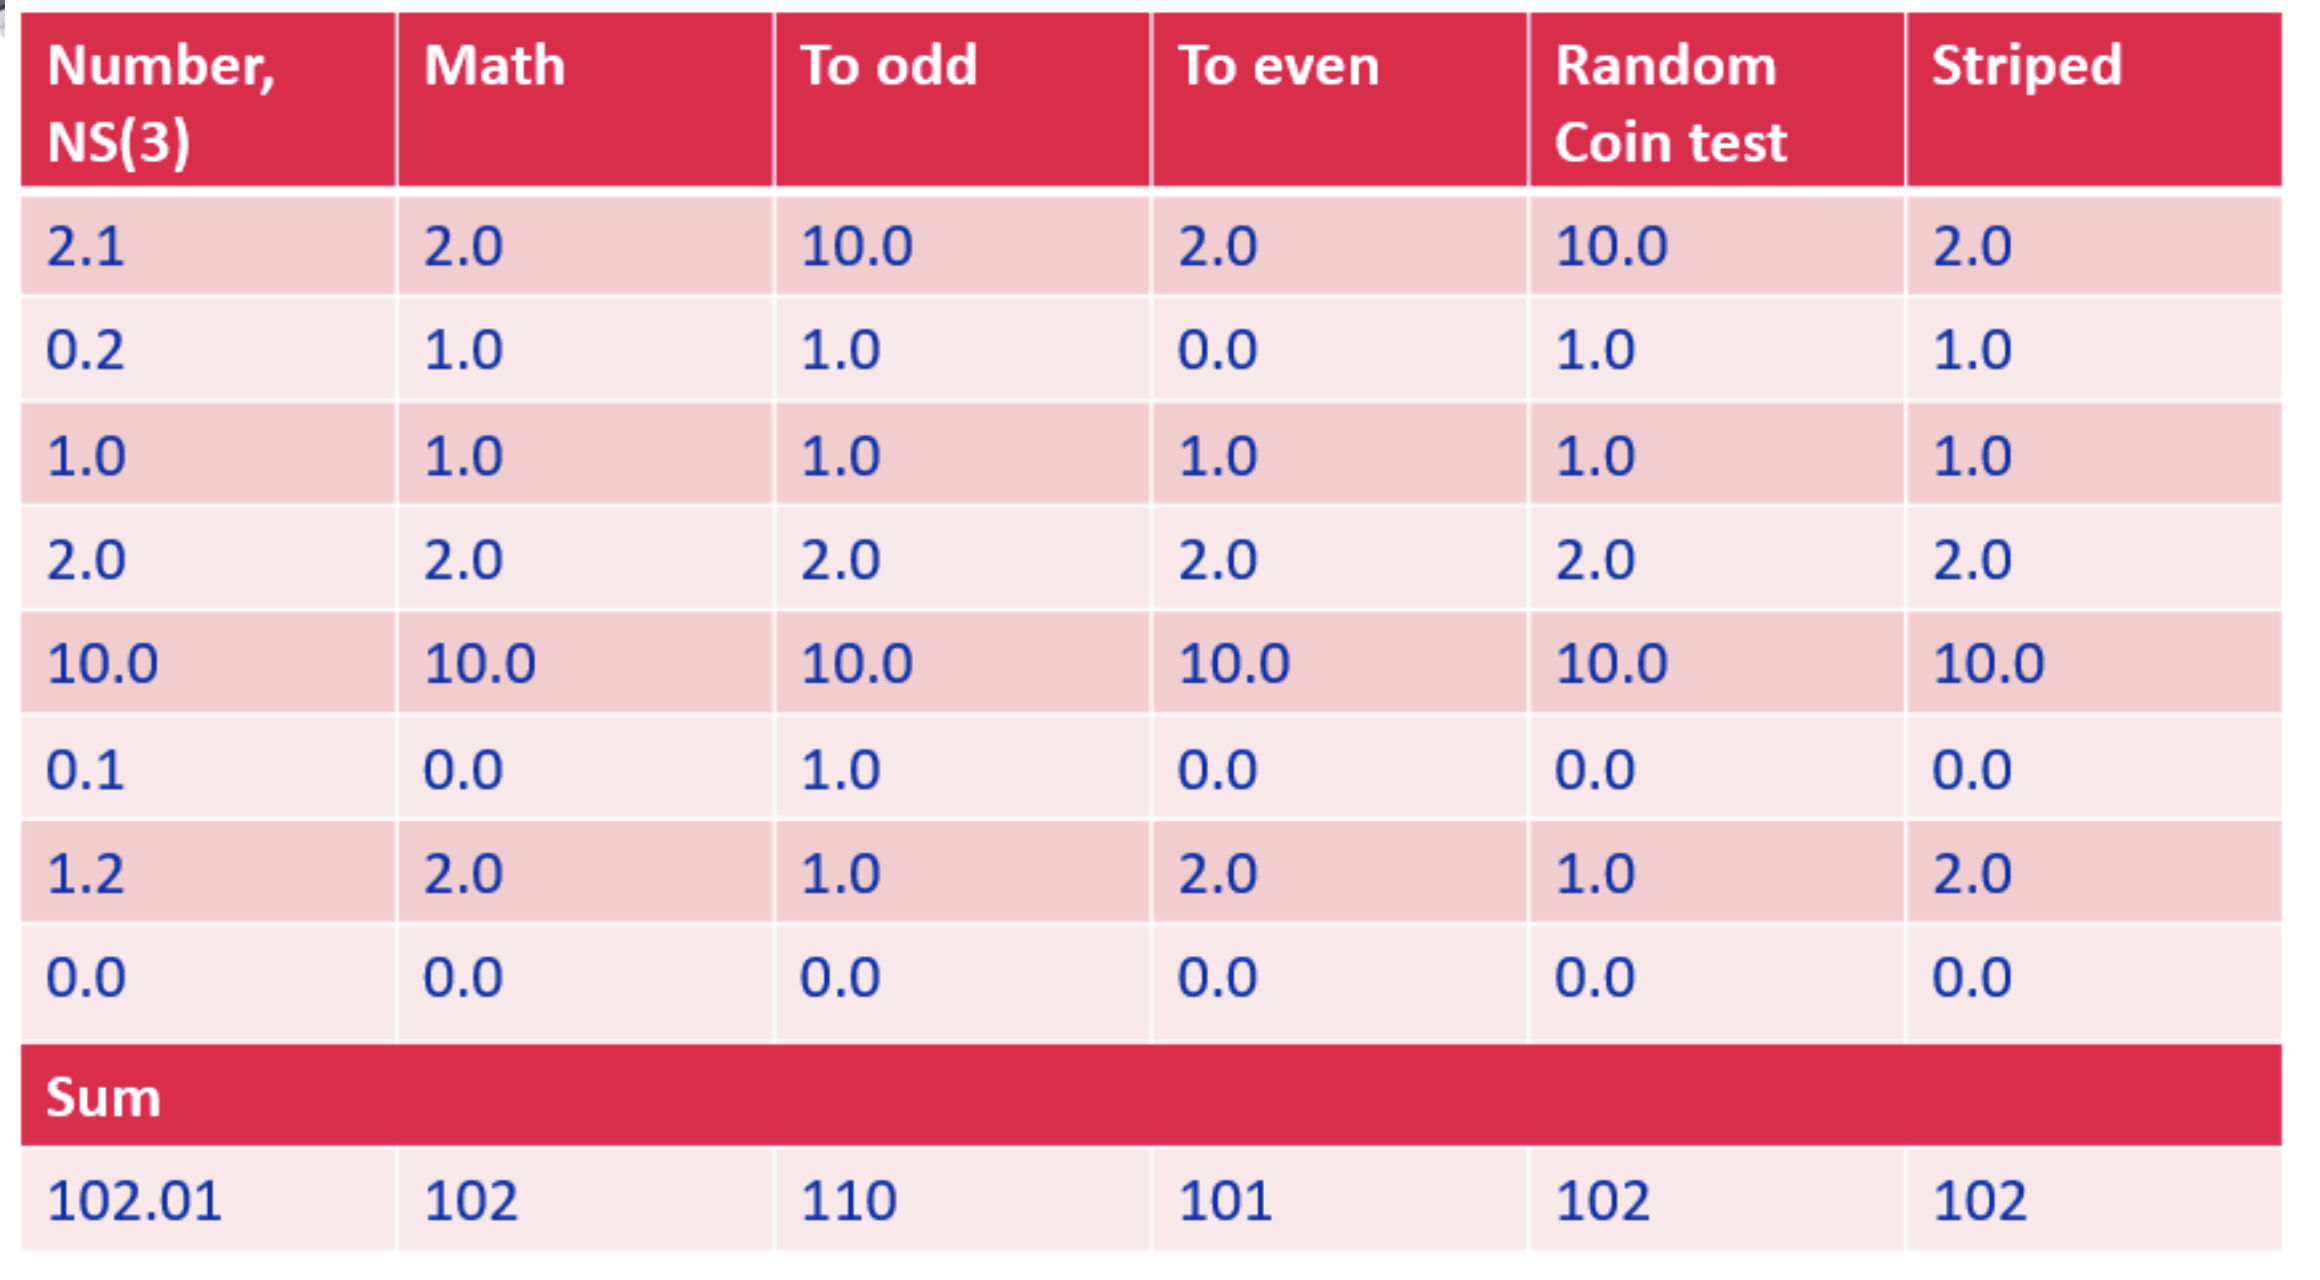
\includegraphics[width=\textwidth]{2.png} % Здесь нужно заменить на реальное изображение
\end{frame}

% Пятый слайд
\begin{frame}{Алфавит и его подмножества}
    \textcolor{custom_green}{Алфавит} – конечное множество различных знаков (букв), символов, для которых определена операция конкатенации (присоединения символа к символу или цепочке символов). \\
    \textcolor{custom_green}{Знак (буква)} – любой элемент алфавита (элемент \(x\) алфавита \(X\), где \(x\inX\). \\
    \textcolor{custom_green}{Слово} – конечная последовательность знаков (букв) алфавита. \\
    \textcolor{custom_green}{Словарь (словарный запас)} – множество различных слов \underline{над} алфавитом.
\end{frame}

% Шестой слайд
\begin{frame}{Кодирование данных}
    \textcolor{custom_green}{Кодирование (модуляция) данных} - процесс преобразования символов алфавита \(X\) в символы алфавита \(Y\). \\
    \textcolor{custom_green}{Декодирование (демодуляция)} - процесс, обратный кодированию. \\
    \textcolor{custom_green}{Символ} - наименьшая единица данных, рассматриваемая как единое целое при кодировании/декодировании. \\
    \textcolor{custom_green}{Кодовое слово} - последовательность символов из алфавита \(Y\), однозначно обозначающая конкретный символ алфавита \(X\) \\
    \textcolor{custom_green}{Средняя длина кодового слова} - это величина, которая вычисляется как взвешенная вероятностями сумма длин всех кодовых слов. \\
    \[L=\sum_{i=1}^{N}p_i*l_i\]
\end{frame}

% Седьмой слайд
\begin{frame}{Кодирование данных (2)}
    Если все кодовые слова имеют одинаковую длину, то код называется \textcolor{custom_green}{равномерным} (фиксированной длины). \\
    Если встречаются слова разной длины, то – \textcolor{custom_green}{неравномерным} (переменной длины).
\end{frame}
\end{document}
